% VI. Disk results (simulated). Every number is a simulated block hit ratio
% of an LRU cache on canonical requests (constraints 1, 13); writes replay as
% reads, and nothing is compared numerically with the MSRC-trace-003 (D17)
% numbers (constraint 5). Hit ratio is always paired with device work (lead
% ruling); belady_min is demand-only MIN, not a bound on prefetching.
% Sources: results/disk/{table_main,table_by_corpus,deltas,kappa}.csv (E1),
% results/gpu/{disk_learned_depth,disk_lstm}.csv (E2), via numbers.tex and
% paper/decisions.py. Generated: Table T2; Fig. F3 (F2, F4, T2b, T2c in the
% appendix).

\section{Disk Results (Simulated)}\label{sec:disk}

% t2_disk_main.tex -- GENERATED by paper/tables/make_tables.py; do not edit.
% Inputs: none
% MISSING input: disk/table_main.csv
\begin{table*}[t]
\centering
\footnotesize
\setlength{\tabcolsep}{3pt}
\caption{Disk results (simulated LRU cache, C1 configuration, canonical requests). Mean block hit ratio over traces; $\Delta$ in percentage points with 95\% paired-bootstrap CIs over traces; device-I/O and blocks-moved ratios are means over traces of the policy's count over \texttt{none}'s. $^\dagger$ gated mode at the break-even cost model. Writes replay as reads.}
\label{tab:t2_disk_main}
\begin{tabular}{l}
\hline
\textbf{MISSING: disk/table\_main.csv} \\
\hline
\end{tabular}
\end{table*}


All numbers in this section are simulated block hit ratios
(Table~\ref{tab:t2_disk_main}).

\textbf{How much to prefetch.} This is the largest lever (P3, P4). Fixed
read-ahead (\texttt{deep@8}) is \decDiskPThreeDeepAtEightAssumedOneMiBVerdict{}
than no prefetching at both capacities
(\decDiskPThreeDeepAtEightAssumedOneMiBPairedCI{} paired and
\decDiskPThreeDeepAtEightAssumedOneMiBClusterCI{} cluster at 1\,MiB, winning on
\diskDeltaHitRatioDeepAtEightVsNoneOneMiBWins{} of \diskDeltaHitRatioDeepAtEightVsNoneOneMiBN{}
traces). In the C2 depth sweep the deepest depth tested
(\diskCTwoDeepest{} blocks) has the highest mean hit ratio in
\diskCTwoBestIsDeepest{} of the \diskCTwoCurves{} corpus--cache curves; only at
1\,MiB do Alibaba and MSR peak earlier, at \diskCTwoBestDepthAlibabaOneMiB{} and
\diskCTwoBestDepthMsrOneMiB{} blocks (Fig.~\ref{fig:f2} in the appendix). In C1,
\texttt{deep@256} adds
\decDiskPThreeDeepAtTwoHundredFiftySixAssumedOneMiBPaired{} at 1\,MiB and
\decDiskPThreeDeepAtTwoHundredFiftySixAssumedSixtyFourMiBPaired{} at 64\,MiB.
Linux-style window growth gets much of that gain with far less waste:
\texttt{linux\_ra@256} adds \decDiskPFourLinuxRaAtTwoHundredFiftySixAssumedOneMiBPairedCI{}
at 1\,MiB, wins on all \diskDeltaHitRatioLinuxRaAtTwoHundredFiftySixVsNoneOneMiBN{}
traces, and leaves \diskWasteLinuxRaAtTwoHundredFiftySixOneMiB{} of its prefetches
unused, against \diskWasteDeepAtTwoHundredFiftySixOneMiB{} for \texttt{deep@256}.
Belady's MIN for demand paging reaches \diskHitBeladyMinOneMiB{} at 1\,MiB
(\texttt{none}: \diskHitNoneOneMiB); several prefetching policies exceed it,
as they may: MIN bounds replacement, not prefetching.

\textbf{Hit ratio is not device work} (P5, P6; Fig.~\ref{fig:f3}). At
1\,MiB, \texttt{deep@8}
\decDiskPFiveDeepAtEightOneMiBVerdict{}
(\decDiskPFiveDeepAtEightOneMiBPairedCI{} of \texttt{none}'s), and
\texttt{deep@256} moves \diskMovedRatioDeepAtTwoHundredFiftySixOneMiB{} as many
blocks. The only policies that reduce device I/Os at either capacity are
\decPFiveReducersOneMiB: window growth merges its reads into larger requests,
so \texttt{linux\_ra@256} needs \decDiskPFiveLinuxRaAtTwoHundredFiftySixOneMiBPairedCI{}
of \texttt{none}'s I/Os at 1\,MiB while moving
\diskMovedRatioLinuxRaAtTwoHundredFiftySixOneMiB{} the blocks; every prefetching
policy moves more blocks than \texttt{none}. Whether that pays depends on the
device: with the measured hard-disk $\kappa$, \texttt{linux\_ra@256}
lowers modelled device time on \diskKappaFavouredSdbLinuxRaAtTwoHundredFiftySixOneMiB{}
of \diskKappaNLinuxRaAtTwoHundredFiftySixOneMiB{} traces and \texttt{deep@8} on
\diskKappaFavouredSdbDeepAtEightOneMiB{} (Fig.~\ref{fig:f4} in the appendix).

\begin{figure}[t]
\centering
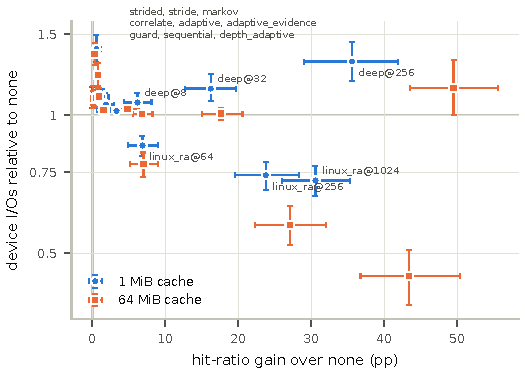
\includegraphics[width=\columnwidth]{figures/f3_device_io_vs_hit}
\caption{Simulated hit-ratio gain over \texttt{none} against device I/Os
relative to \texttt{none}, C1, both cache sizes, with paired \ciLevel{}
bootstrap intervals over the \diskTraces{} traces. Only window growth lies below
one.}
\label{fig:f3}
\end{figure}

\textbf{The learned class router.} The classifier-routed \texttt{adaptive}
policy is \decDiskPOneAdaptiveAssumedOneMiBVerdict{} than \texttt{sequential} at
both capacities (P1): \decDiskPOneAdaptiveAssumedOneMiBPairedCI{} paired and
\decDiskPOneAdaptiveAssumedOneMiBClusterCI{} cluster at 1\,MiB, losing on
\diskDeltaHitRatioAdaptiveVsSequentialOneMiBLosses{} of
\diskDeltaHitRatioAdaptiveVsSequentialOneMiBN{} traces, and
\decDiskPOneAdaptiveAssumedSixtyFourMiBPairedCI{} at 64\,MiB (losing on
\diskDeltaHitRatioAdaptiveVsSequentialSixtyFourMiBLosses). It still beats
\texttt{none} (\diskVsNoneAdaptiveOneMiBCI), but by less than the two-block
read-ahead it routes between, and with more device I/Os
(\diskIORatioAdaptiveOneMiB).

\textbf{The feedback gate.} Against \texttt{sequential}, \texttt{guard} is
\decDiskPTwoGuardAssumedSixtyFourMiBVerdict{} at 64\,MiB
(\decDiskPTwoGuardAssumedSixtyFourMiBPairedCI) and at 1\,MiB its result is
``\decDiskPTwoGuardAssumedOneMiBVerdict'' (paired
\decDiskPTwoGuardAssumedOneMiBPairedCI, cluster
\decDiskPTwoGuardAssumedOneMiBClusterCI). At the break-even cost model it is
\decDiskPTwoGuardBreakEvenOneMiBVerdict{} at both capacities and stays within
\diskBreakEvenVsNoneGuardOneMiB{} of \texttt{none}. The gate limits waste and device
work (\diskIORatioGuardOneMiB{} of \texttt{none}'s I/Os, against
\diskIORatioSequentialOneMiB{} for \texttt{sequential}) but adds no hits over
\texttt{sequential}.

\textbf{Which lever is smallest.} The pre-registered ordering compares the
intervals of $|\Delta|$ against \texttt{sequential}. At 1\,MiB the predictor
(\decDiskOneMiBPredictorSmallestPredictorPairedCI{} pp paired) and the
feedback gate (\decDiskOneMiBPredictorSmallestFeedbackPairedCI) cannot be
ordered; both are smaller than depth
(\decDiskOneMiBPredictorSmallestDepthPairedCI) and window growth
(\decDiskOneMiBPredictorSmallestWindowGrowthPairedCI), and depth is smaller than
window growth, in both the paired and the cluster intervals. At 64\,MiB the
order is complete: feedback, then the predictor, then depth, then window
growth. So the rule's verdict at both capacities is that
\decDiskSixtyFourMiBPredictorSmallestVerdict: the learned predictor moves the
hit ratio little, but the feedback gate moves it as little or less.

\textbf{Robustness.} Of the \decTallyCThree{} P1--P4 decisions that C3 repeats,
\decTallyCThreeRobust{} are \emph{robust} on a second slice of the subset traces;
\texttt{deep@32} against \texttt{none} is
\decDiskCThreeDeepAtThirtyTwoAssumedVerdict{} (better on the first slice,
paired-only on the second). On FIU, \decTallyCFourCapInsensitive{} of
\decTallyCFour{} are cap-insensitive between merge caps of 256 and 1024
sectors. Request reconstruction matters a great deal: on FIU at C2,
\texttt{deep@8} gains \diskDeltaFiuCTwoHitRatioDeepAtEightVsNoneOneMiBCI{} on merged
requests but \diskDeltaFiuCTwoNoneHitRatioDeepAtEightVsNoneOneMiBCI{} on the unmerged
4\,KiB page records, an artefact of counting each page as a request that we
report only as a sensitivity view.

\textbf{Learned depth and the LSTM.} The GPU-trained depth controller is
\decDiskLearnedDepthVsVcfCapTwoHundredFiftySixVerdict{} than the
validation-chosen fixed depth at both action caps, on held-out test segments:
\decDiskLearnedDepthVsVcfCapSixtyFourPairedCI{} with a 64-block cap (cluster
\decDiskLearnedDepthVsVcfCapSixtyFourClusterCI; it wins on
\ldVsVcfCapSixtyFourWins{} of \ldVsVcfCapSixtyFourN{} traces) and
\decDiskLearnedDepthVsVcfCapTwoHundredFiftySixPairedCI{} with a 256-block cap,
over \ldSeedsCapTwoHundredFiftySix{} seeds. The GPU study records prefetches,
not device I/Os: the controller issues \ldIssuedVsVcfCapSixtyFour{} and
\ldIssuedVsVcfCapTwoHundredFiftySix{} as many as VCF under the two caps. It does beat \texttt{deep@8}
(exploratory; \ldVsDeepEightCapTwoHundredFiftySixCI), but \texttt{deep@8} is not the fair
baseline: the depth a validation split chooses is. The LSTM predicts address deltas, so we compare only its
cache outcome: on its \lstmTraces{} traces its mean test hit ratio
(\lstmMeanHit) is below \texttt{linux\_ra}'s (\lstmMeanLinuxRaHit) on
\lstmBelowLinuxRa{} of \lstmTraces{} and close to \texttt{none}'s
(\lstmMeanNoneHit); its contended GPU timings are not quoted.
